% Chapter 3

\chapter{Onderzoeksmethode}\label{ch:onderzoeksmethode} % Chapter title

Zoals in de inleiding vermeld zijn er twee onderzoeken benodigd om deze opdracht te kunnen volbrengen.
In de komende secties is te vinden welke methode, stategiën en scoping zijn gebruikt om een resultaat te vinden.
Waarbij iedere sectie een onderzoek vertegenwoordigd


\section{Onderzoek: Architectuur binnen Eaglescience}\label{sec:onderzoeksmethode-architectuur-binnen-eaglescience}
Het resultaat van dit onderzoek moet zijn: "Het hebben van inzicht in de manier van werken binnen Eaglescience en de daarbij horende keuzes voor ontwikkeltalen, architectuur, en tools".
Om deze inzicht te krijgen is het volgende onderzoeksmodel (figuur:\ref{fig:Onderzoeks model Eaglescience}) opgesteld waarbij er vanuit eigen kennis, interne workshops en vooronderzoek gekeken is naar gebruikte ontwikkelingstalen en tooling.
Deze is vervolgens geverifieerd met senior developers.
Hieruit is vervolgens het resultaat in de vorm van inzicht in de huidige dev-stack naar voren gekomen.
\begin{figure}[h!] %todo: Nog in kleur zetten van Eaglescience als deze goed is.
  \myfloatalign
  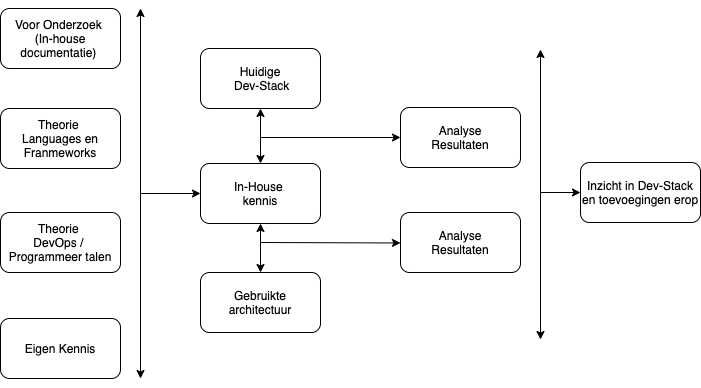
\includegraphics[width=10cm]{gfx/OnderzoeksmodelES}
  \caption{Onderzoeksmodel Eaglescience}
  \label{fig:Onderzoeks model Eaglescience}
\end{figure}

Zoals vermeld is er eerst vanuit eigen kennis, vooronderzoek en kennis opgedaan in de door Eaglescience workshops een lijst gemaakt met de gebruikte technieken.
Daarna is deze geverifieerd met senior ontwikkelaars doormiddel van interviews.
Tijdens deze interviews is ook ruimte geweest voor de reden en filosofie achter de keuzes die er gemaakt zijn in het gebruik van de talen.

\section{Onderzoek naar SOUP-analyse}\label{sec:onderzoek-naar-soup-analyse}
Dit onderzoek heeft als ingang het gegeven dat er kwetsbaarheden in de bibliotheken zitten met daarbij de dev-stack van Eaglescience.
Het resultaat van dit onderzoek moet zijn dat er een methode moet zijn waarbij er een assesment op de bestaande dev-stack binnen de werkwijze van Eaglescience moet komen die geimplementeerd kan worden.
Het onderzoekmodel (figuur:\ref{fig:Onderzoeks model Dev-Stack}) geeft weer dat de ingangs kennis de opgedane kennis uit het onderzoek naar de architectuur van Eaglescience en een literatuur studie naar mogelijkheden om soup te analyseren.

\begin{figure}[h!] %Todo: Nog in kleur zetten van Eaglescience als deze goed is.
  \myfloatalign
  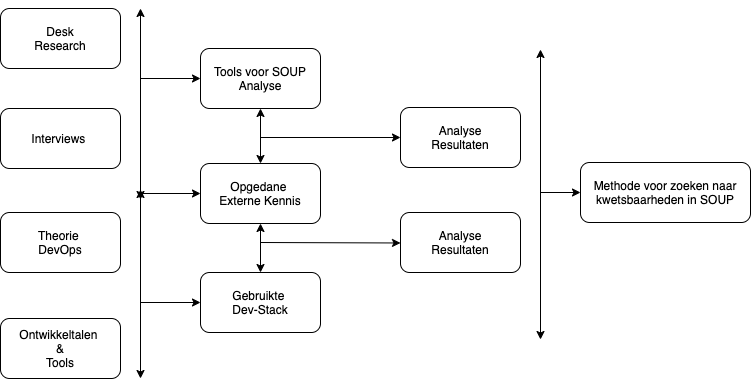
\includegraphics[width=10cm]{gfx/OnderzoeksmodelSOUP}
  \caption{Onderzoeksmodel SOUP analyse module}
  \label{fig:Onderzoeks model Dev-Stack}
\end{figure}

Veel kennis van buiten zal worden vergaard doormiddel van het lezen van artikelen en boeken over het onderwerp.
Hierbij moet worden gelet op de toepasbaarheid en scope van het artikel.

\section{Tijdsverloop Onderzoeken}\label{sec:tijdsverloop-onderzoeken}
Beide onderzoeken zullen parallel uitgevoerd worden zodat beide onderzoeken elkaar inzichten kunnen verschaffen en er op die manier een beter begrip van de mogelijkheden is.
